\chapter{Idea of Photometry}

\section{The Point-Spread Function (PSF)}

Stars must be point sources. But from our experience, we know that they are never a point, but a usually nearly circular extended sources on the CCD. The image on the CCD when a single perfect point source is imaged, is called the \textbf{point spread function (PSF)}. There are basically two mechanisms responsible for this: diffraction and seeing. Although diffraction can also be a part of seeing, it is somewhat special than others: It is just impossible to eliminate the diffraction, while other sources of seeing can be removed (see below).

\subsection{Diffraction}
When a light ray passes through a finite-sized aperture, diffraction must occur. Due to this, a point source is blurred to a finite size after it passed through an aperture (e.g., telescope or DSLR camera aperture). 

\begin{ex}[Diffraction]
	For $ D = \SI{1}{m} $ in visible ($ \SI{550}{nm} $ wavelength), the diffraction limit is $ 1.22 \frac{\lambda}{D} = \SI{0.14}{arcsec}$. You may be familiar with this formula. Using the proportionality, you can memorize it as $ \theta_\mathrm{min}^{(\SI{550}{nm})} = \frac{0.14}{D\mathrm{[m]}} \mathrm{arcsec}$.
\end{ex}

It is more complicated in reality: the mirrors and other optical instruments located in the optical path affect the final shape of a point source by diffractions. See \cref{fig:psftelescopes} for the examples of simulated PSFs from optics, i.e., when the seeing effects are neglected.

\begin{figure} [htb!]
	\centering
	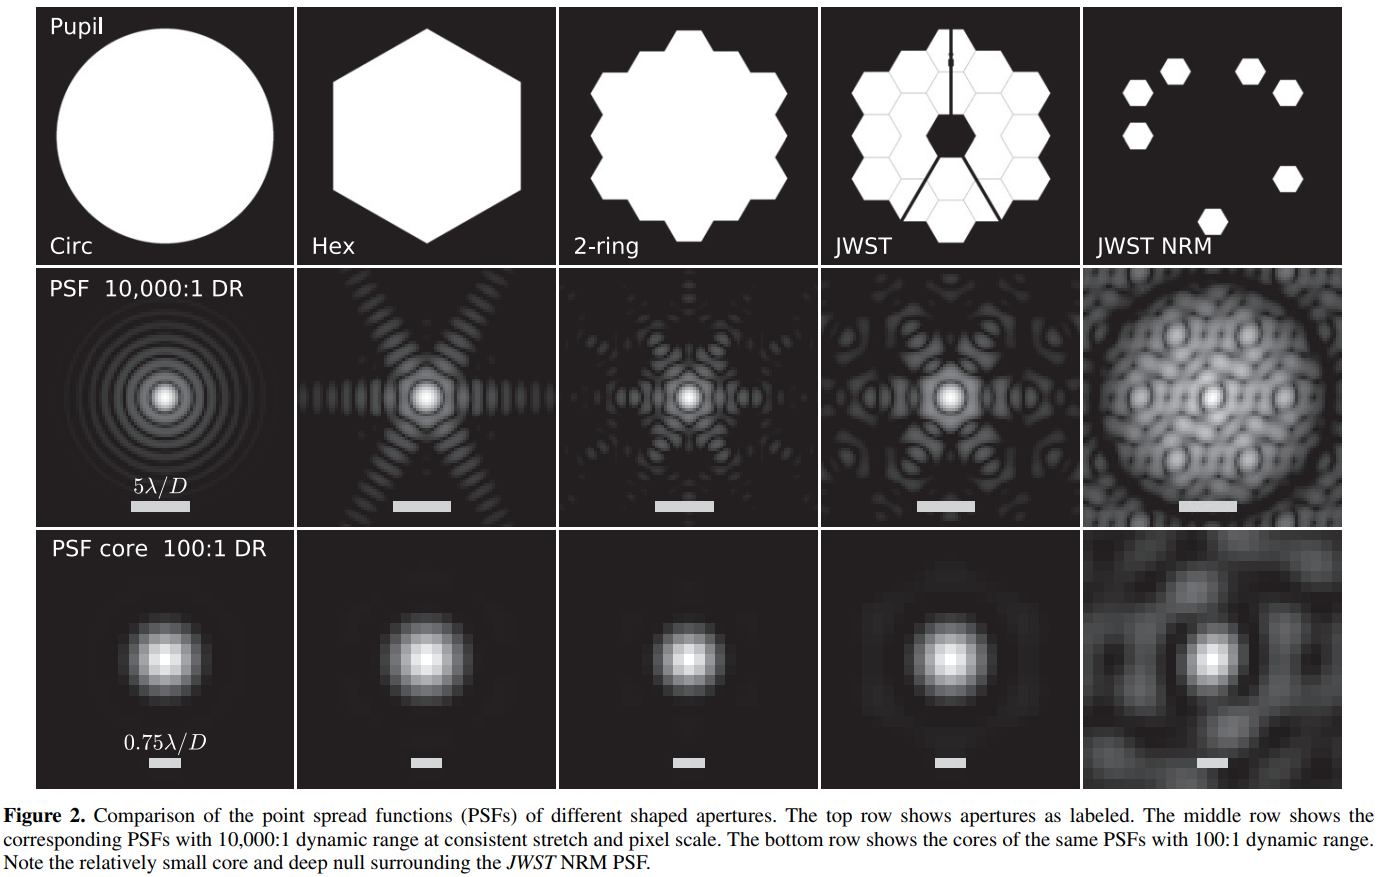
\includegraphics[width=0.9\linewidth]{figs/psf_telescopes}
	\caption{Example of PSFs. For circular aperture, the PSF shows concentric diffraction pattern as we learned in general physics course. For JWST case, you can see the secondary mirror and the mirror holding pipe (black things) makes the PSF different compared to the 2-ring case. The bottom row is not just a zoom-in of the PSF, but also the stretch (contrast) is different from the mid row (DR means the dynamic range). Direct excerpt from Figure 2 of FordKES+, 2014, ApJ, 783, 73.}
	\label{fig:psftelescopes}
\end{figure}

As you can see in \cref{fig:psftelescopes}, although the detailed PSF are different (mid row), the long-range features are weaker compared to the central nearly circular features (bottom row) in cases except for the last column, which is not of our interest. 


\subsection{Seeing}

Even if we ignore the diffraction, a point source is blurred due to two main reasons: (1) air turbulence and (2) discontinuous movement of the telescope since the telescope gear is not a perfectly smooth continuous ideal machine. The blurring caused by these are called \textit{natural (atmospheric)} and \textit{telescopic seeing}, respectively. The atmospheric seeing makes a point source an extended circular source (for details, search for the theory of, e.g., Andrei Kolmogorov), while the telescope seeing \textit{may} make it very elongated or irregular depending on the quality of the tracking system. If the tracking system is well established on a telescope, the final telescope seeing effect is quite circular. 

All these effects can be removed if we move our telescope in space. The atmospheric turbulence is now gone, and the telescope can be very stable such that the telescopic seeing is ignorable. This is what is called the diffraction-limited case.


\subsection{Summary of PSF}

To summarize:
\begin{align*}
  \mathrm{PSF} &= \mathrm{diffraction} + \mathrm{seeing} \\
  \mathrm{seeing} &= \mathrm{atmospheric~seeing} + \mathrm{telescopic~seeing}
\end{align*}
and practically speaking,
\begin{equation*}
  \mathrm{PSF~shape} \approx \mathrm{circular} ~.
\end{equation*}
This is why we can talk about the circular aperture photometry. Also
\begin{align*}
  &\mathrm{diffraction} \ll \mathrm{other~sources~of~seeing} \\ &\mathrm{(unless~adaptive~optics~or~space~telescope~used)} ~.
\end{align*}

Actually, for many ground-based observations, it is not necessarily important to distinguish diffraction from other seeing effects. I feel like people tend to use the word ``PSF'' when the PSF is measured rather accurately (e.g., PSF photometry), and use the word ``seeing'' when we assumed circular PSF (e.g., aperture photometry). 

\subsection{Seeing Disc Size}
As mentioned above, when we assume circular PSF (as we will do frequently in aperture photometry), we use the word ``seeing'' for the PSF. \textit{Seeing disc} is the word for the circular shape of the PSF, and the \textit{seeing disc size} is a measure of the size of that circle. The definition of the ``size'' is not trivial, but many people use the FWHM of the stellar radial profile\footnote{Radial profile means the pixel values of the star image as a function of the distance from the center of the star: $ I(r) $. From many free/commercial products, it is rather easily drawn, such as \texttt{ginga}, \texttt{SAO ds9}, or \texttt{Maxim DL 6}. They also automatically calculates FWHM for you. The details on how to find the ``center'' will be studied later. Here, just think about something like Gaussian curve.}. This seeing disc size measurement is used to find the focal position and give a sense to the data quality.

The seeing disc FWHM is dependent on wavelength, weather, airmass, etc. At Seoul National University observatories in Seoul, it is roughly 1 to 3 arcsec at Bldg. 46 and 3 to 6 arcsec at Bldg. 45. For Subaru telescope at Hawai'i, for example, it is less than 1 arcsec\footnote{\url{https://www.naoj.org/Observing/Telescope/ImageQuality/Seeing/}}. Compared to the diffraction size $ \theta_\mathrm{min} $, these are much larger. It can go even below if we use adaptive optics (then $ \mathrm{diffraction} \approx \mathrm{total~seeing} $ and non-circular PSF may be important).

The fact that the seeing disc size (i.e., size of the circular PSF) on the CCD is normally much larger than the diffraction scale hint that atmospheric and telescope seeing are very important. Since the telescope seeing is roughly constant over time for continuous tracking of a good telescope, the change in seeing can also strongly dependent on the weather condition. So astronomers use seeing disk size (usually rough estimate of FWHM) as a proxy of the weather condition.

It can also be used as a data-quality-indicator.

\begin{ex}[Contamination by Other Object]
If you have your faint target near a bright stellar source with 1 arcsec separation and if the seeing disc FWHM is roughly 1 arcsec, your faint target is contaminated by the nearby bright star. A possibility is to do photometry of ``your target $ + $ bright star'' and subtract the flux of the ``bright star'' from catalog or future/previous observations. In this case, although you can get the flux of the target, its uncertainty may increase significantly. 
\end{ex}

\begin{ex}[Slit Width Determination]
For spectroscopy, seeing disc size may determine the slit width you have to use to collect the target's light into the slit. It will be dealt in the spectroscopy chapter.
\end{ex}

\begin{ex}[Finding Focal Position from Seeing FWHM]
First find a random bright star that do not vary over short period of time (e.g., about 1 hour). You then expose and check the FWHM of the PSF (assuming it is circular). Now tune the focal position, e.g., by moving the position of the secondary mirror, and expose again, and check the FWHM again. Doing this repeatedly, you can get the FWHM as a function of the focal position. When the FWHM becomes the minimum, that is \textit{the} focal position (\cref{fig:focusing}). Normally this curve is roughly second order polynomial.
\end{ex}

\begin{figure}[ht!]
  \centering
  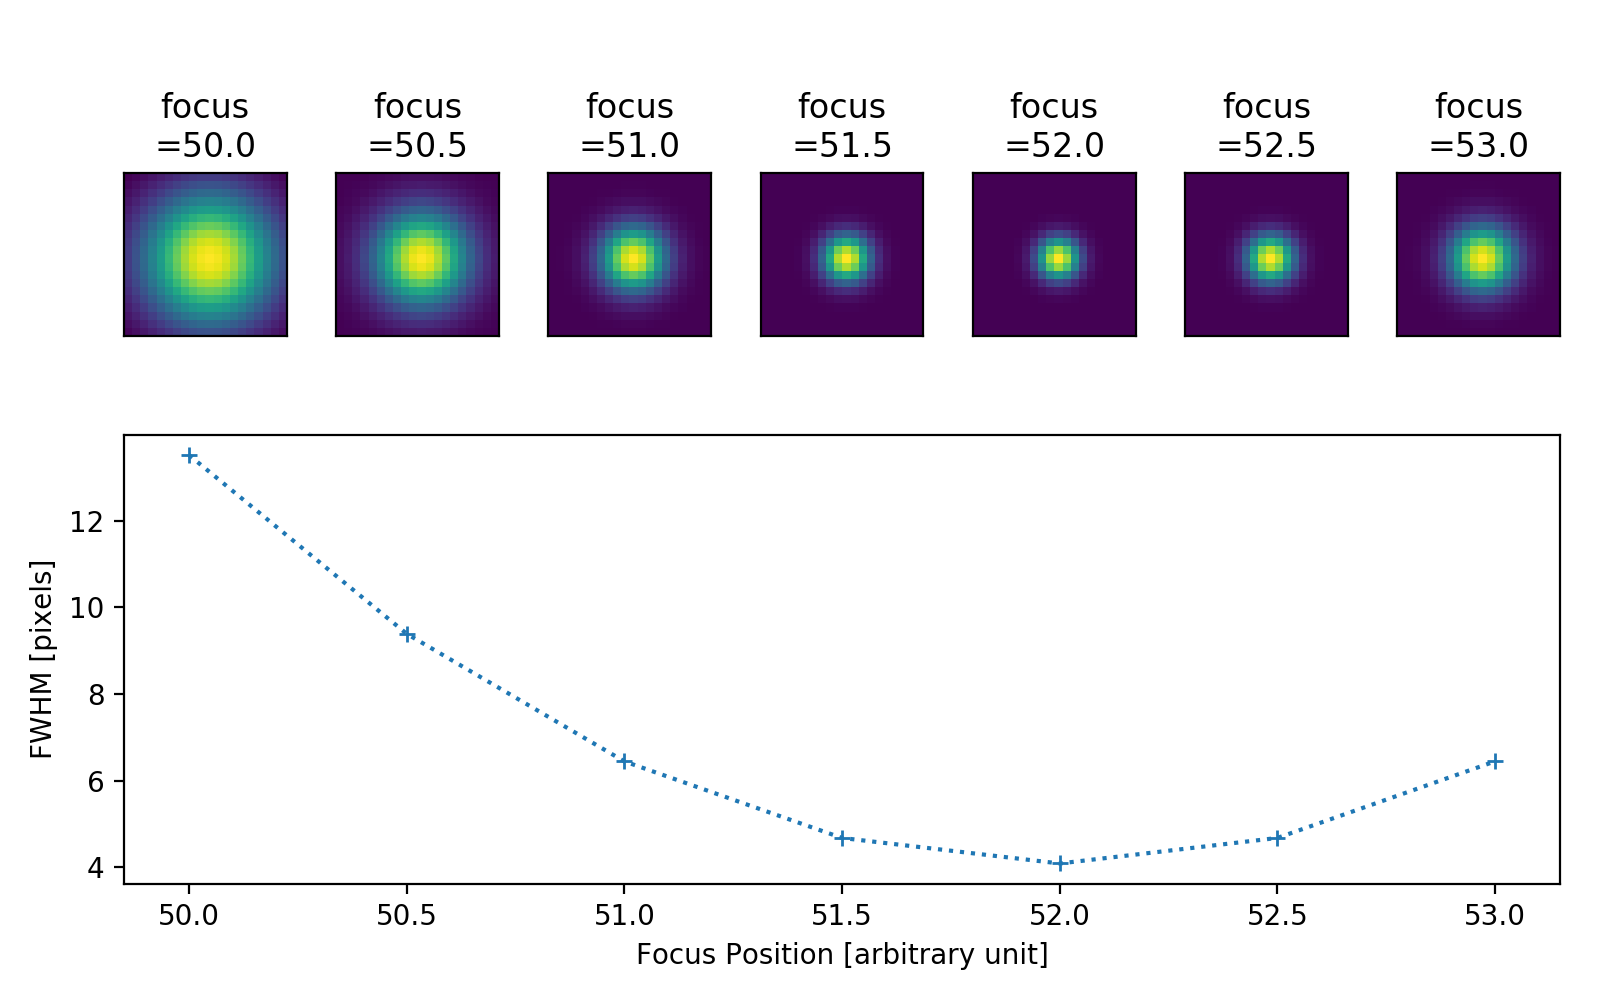
\includegraphics[width=0.7\linewidth]{figs/focusing}
  \caption{Finding focal position. While tuning the focal position value (x-axis), check the FWHM of the stellar profile. In this fake simulation, it is found that the focal position of 52.0 is \textit{the} focal position with FWHM $ \sim 4 $ pixels. Multiplying with the pixel scale will give the FWHM in angular units (e.g., if the pixel scale is $ \SI{0.8}{arcsec/pixel} $, FWHM after the focusing is $ \SI{4}{pixel} \times \SI{0.8}{arcsec/pixel} = \SI{3.2}{arcsec} $)}
\label{fig:focusing}
\end{figure}


Our goal in observation is to ``gather all the photons from the target''. For a faint source, you have to tune the focal position very accurately, so that the signal from the source gathers to as small number of pixels as possible. Otherwise, the signal will be buried in sky values or other noise sources (dark current or readnoise) and our goal may not be achieved. The non-circular PSFs for high-quality data shares this same philosophy: the ``sprays'' of PSF should be analyzed. But for a very bright source, you may even intentionally defocus before the exposure. This is because we can avoid saturation and blooming from the central pixels while the signal is so strong that the noise is overwhelmed by the source signal. Then our goal is achieved even if we forget about the accurate focal position or accurate PSF.


\section{Centroid}
Even though we know the accurate PSF, we cannot use it for photometry if we cannot determine the center or the origin. There are various ways to determine this ``origin'', but the most widely used one is centroiding (center of mass). 

%but most of them have one or more of the following drawbacks: (1) no analytic solution but numerical calculation needed, (2) computationally heavy, (3) formulated only by empirically. One of the useful analytical centroiding is given here.

Let $ I_i $ for $ i = 1, 2, \cdots , N $ means the $ i $-th pixel with $ (x, y) = (x_i, y_i) $ of the original $ N_x \times N_y $ 2-D pixel array so that $ N = N_x N_y $. Say we set a threshold $ I_0 $ (e.g., background value, signal-to-noise ratio of 3, etc). Then change $ I_i = 0 $ if $ I_i < I_0 $. For $ \xi = x $ or $ y $, the centroid is by definition
\begin{equation} \label{eq: centroid}
  \xi_c = \frac{\sum_i I_i \xi_i}{\sum_i I_i} ~.
\end{equation}
By using the error-propagation, the uncertainty of $ \xi_c $ is, considering $ \xi_i $'s are fixed with no uncertainty,
\begin{equation}
  \qty (\Delta \xi_c)^2
    = \qty(\pdv{\xi_c}{I_1})^2 \qty(\Delta I_1)^2 
      + \cdots + \qty(\pdv{\xi_c}{I_N})^2 \qty(\Delta I_N)^2 ~.
\end{equation}
But
\begin{equation}
  \pdv{\xi_c}{I_k} 
    = \pdv{I_k} \qty( \frac{I_1 \xi_1 + \cdots + I_N \xi_N}{I_1 + \cdots + I_N} )
    = \frac{\xi_k}{\sum_i I_i} - \xi_c ~,
\end{equation}
so
\begin{equation}
  \qty (\Delta \xi_c)^2
  = \sum_k \qty(\frac{\xi_k}{\sum_i I_i} - \xi_c)^2 \qty(\Delta I_k)^2
  = \frac{\sum_k (\xi_i - \xi_c)^2 \qty(\Delta I_k)^2}{\sum_i I_i} ~.
\end{equation}
Pixels near the object are likely to have high pixel values, so we approximate the uncertainty $ \Delta I_i $ is just the Poisson noise of the pixel value (which is source $ + $ sky $ + $ read noise), i.e., \cref{eq: Pois mean std}, $ \Delta I_i = \sqrt{I_i} $. Then expanding the square and using the definition of $ \xi_c $, we get
\begin{equation} \label{eq: centroid err}
  \Delta \xi_c 
  = \sqrt{\frac{\sum_k (\xi_i - \xi_c)^2 I_k }{\sum_i I_i} }
  = \sqrt{\frac{s_c^2}{\sum_i I_i}}
\end{equation}
where
\begin{equation}
  s_c^2 = \frac{\sum_k \xi_k^2 I_k}{\sum_i I_i} - \xi_c^2 ~.
\end{equation}


There are some other techniques which involves Gaussian fitting: marginalize the image onto the $ x $- and $ y $-axes, and do the 1-D Gaussian fitting to each of them. Also the sigma-clipping inside the centroiding box (cbox) can be used (e.g., Ma+ 2009, Opt.Exp., 17, 8525).

\section{Aperture Sum}
We need first to find the total flux inside the aperture. The sky subtraction will be done later. Consider a very simple case in \cref{fig:photapex01}: The centroid is calculated following \cref{eq: centroid}, and it is trivial that the centroid is at the center of the shown image. If we put circular aperture of radius 1 pixel (middle panel), the pixel contribution from the pixel with value 10 (right panel) is
\begin{equation}
  \mathrm{pixel~value} \times \frac{\mathrm{area~in~aperture}}{\mathrm{total~area}}
  = 10 \times \frac{\pi / 4}{1}
  = 7.854 ~.
\end{equation}
Doing the same calculation for all the 4 pixels inside the aperture, you will get $ N_\mathrm{apsum} = 47.12 $, where apsum means the ``aperture sum''. 

\begin{figure} [ht!]
\centering
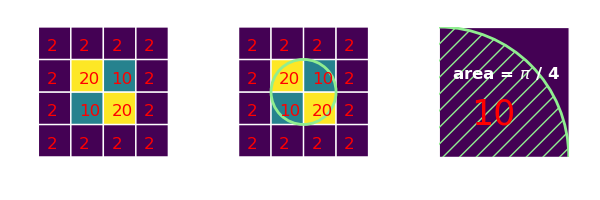
\includegraphics[width=0.7\linewidth]{figs/phot_ap_ex01}
\caption{Left: An example pixel values near the source. Middle: An aperture of radius 1 pixel shown as green circle. Right: A zoom in of one pixel with pixel value 10.}
\label{fig:photapex01}
\end{figure}

One thing to note is the uncertainty in position. In this 4 by 4 pixel example, $ \sum_i I_i = 84 $ and $ \xi_c = (x_c, y_c) = (1.5, 1.5) $ under the 0-indexing. For $ \Delta x_c $, we consider only the $ x $-coordinate for \cref{eq: centroid err} caluclation. Note that in that case, $ \sum_k (x_k^2 I_k) $ for all the $ \num{4 x 4} = 16 $ pixels is nothing but $ \sum_{k=1}^{4} (x_k^2 I'_k) $ where $ I' = [8,\, 34,\, 34,\, 8] $ is the marginalized intensity along the $ x $ direction from \cref{fig:photapex01}. Then $ \Delta x_c = 0^2 \times 8 + 1^2 \times 34 + 2^2 \times 34 + 3^2 \times 8 = 242 $. This must be the same for the $ y $-axis, and thus $ s_c^2 = 242 / 84 - 1.5^2 = 0.63 $, so $ \Delta x_c = \Delta y_c = \sqrt{0.63 / 84} = 0.087 $ pixel.

Here, I did not touch the topics such as (1) how to select the aperture radius, $ r_\mathrm{ap} $ and (2) in reality, we need to fit some function to the radial profile, but which function should we use? These will be dealt in the next chapter.

Since this aperture sum includes not only the source but also the sky values (sky value is always non-zero for ground-based observations), we need to subtract the sky.


\section{Sky Estimation}
Estimation of the sky is one of the most trickest part in observational astronomy. There are two most widely used methods: annulus and 2D interpolation. I will first explain few formulae, and then explain these two methods.

\subsection{Simple Parametric Sky Estimation}
There have been some parametric methods to estimate correct sky value. The most widely used ones include the ``MMM'' relation, or the ``mean-median-mode'' relation, and regard the mode (most frequent value) as the constant sky value. This has been used by virtually all astronomical softwares, including IRAF, IDL, SExtractor, and python packages. It is the simplest and does not require much computational speed, while gives reasonable results in many cases.

Why mode? The mission in determining the \textit{constant} sky value is to find a \textit{robust}, i.e., trustful constant value. Average (mean) is very vulnerable to few outliers even though we did sigma-clipping, and the median is less robust than mode, because if faint object with $ S/N $ ratio $ \sim 1 $ is in the sky region, the median can also be overestimate the sky. Thus, mode is the most widely used simple statistic for sky estimation.

The determination of the modal value is very difficult, because the it is not simple to define it for the \textit{sampled data}. If the distribution is not a mathematically continuous one, i.e., if it is discrete as we always encounter after sampling process, the mode is the largest value when we draw a \textit{histogram}. The histograms are basically sensitive to the subjective selection of bins, and you can change the modal value to an unexpected value depending on the bin you choose (see \cref{fig:phottestsky01}). %It gets very complicated because the pre-processed image can have real number values, not integers. Hence, the histogram may look like a comb with only 1 count at each comb, if the bins are set to be infinitesimally small. 

\begin{figure}[ht!]
\centering
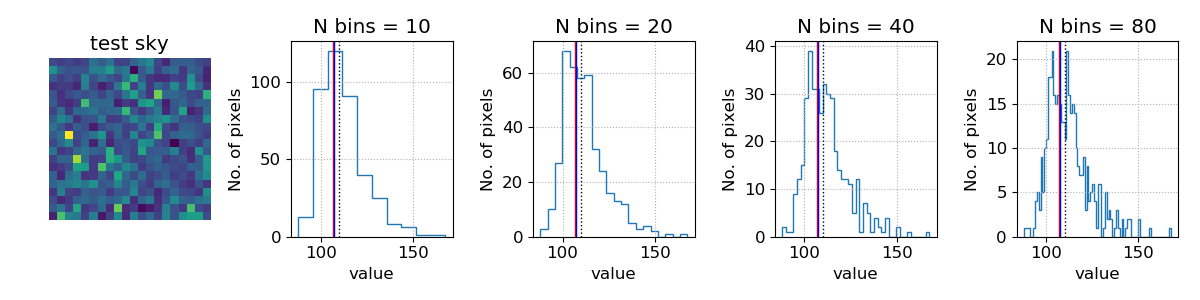
\includegraphics[width=\linewidth]{figs/phot_testsky01}
\caption{Left: A fake sky of 20 by 20 pixels generated by $ 100 + \mathcal{N}(0, 5^2) + 5 \chi^2_2 + 3 \mathcal{U}(0, 1) $ (normal distribution, chi-squared distribution, and uniform distribution, respectively). Others: The histogram of the pixel values with different bin numbers with fixed bin width. The black dotted lines is the median, and the red and blue solid lines are the mode estimation from \cref{eq: mmm 3 2,eq: mmm sex}, respectively (almost indistinguishable). As can be seen, the mode value does not lie at the same position, and it even become bimodal when the number of bins is 80.}
\label{fig:phottestsky01}
\end{figure}

Since 1800s, people empirically knew that the mode has the following relationship which holds for a moderetely asymmetric distribution:
\begin{equation}\label{eq: mmm 3 2}
  \mathrm{mode} \approx 3 \times \mathrm{median} - 2 \times \mathrm{mean} ~,
\end{equation}
or equivalently, \textit{the distance between the mode and median is two-thirds of that between mode and mean}. DoodsonAT (1917, Biometrika Trust, 11, 425) first gave mathematical proof of it using some mathematical tricks including Laplace's and De Morgan's (1836), and it is recognized by many statisticians including KendallMG (1943; or the second edition of it in 1945, The Advanced Theory of Statistics 2e, Vol 1, p.35). People now refer to more recent references like KendallMG+StuartK (1977, The Advanced Theory of Statistics, Vol. 1. Charles Griffin \& Co., London).

SExtractor (BertinE+ArnoutsS, 1996, A\&AS, 117, 393) uses a variant of this:
\begin{equation}\label{eq: mmm sex}
  \mathrm{mode} \approx 2.5 \times \mathrm{median} - 1.5 \times \mathrm{mean} ~.
\end{equation}
There is no clear reason provided in the original paper nor the SEx user manual, but it is just descibed that it was found to be more accurate when they tested. The estimation process works like this: Get the mean, median, and sample standard deviation (mean, med, std, respectively) from the sky pixel values after sigma-clipping. If $ \frac{\mathrm{mean} - \mathrm{med}}{\mathrm{std}} > 0.3 $, use $ \mathrm{mode} \approx \mathrm{med} $\footnote{Although the publication and SEx manual says they use mean if $ \frac{\mathrm{mean} - \mathrm{med}}{\mathrm{std}} > 0.3 $, but the SEx software actually returns med, not mean (described in photutils v0.6, Background Estimation (photutils.background))}. Otherwise, use \cref{eq: mmm sex}. 

IDL MMM uses \cref{eq: mmm 3 2}. IRAF also uses \cref{eq: mmm 3 2} internally, but it gives the mean value if $ \mathrm{mean} < \mathrm{med} $. In astropy-related packages (e.g., \texttt{photutils}), it is the user's choice. In all cases, you can set the sigma-clipping factors, e.g., $ a $ such that data outside $ \mathrm{med} \pm a \times \mathrm{std} $ can be rejected, and $ n $, the maximum iterations this process should be done until no more data are rejected. Whether to use $ \mathrm{med} \pm a \times \mathrm{std} $ or $ \mathrm{mean} \pm a \times \mathrm{std} $, whether to give asymmetric $ a $ values (upper and lower sigma-clipping), etc are up to the user.

I recommend to follow what SEx does, with sigma-clipping of $ a \sim 3 $ and $ n \ge 5 $, because that became a virtual standard in parametric sky estimation.


\subsection{Other Ways for Sky Estimation}
As can be seen from \cref{fig:phottestsky01}, the sky histogram is mostly skewed towards right. Because of this, BijaouiA (1980, A\&A, 84, 81) first introduced to fit the sky histogram with Gaussian multiplied by Laplace:
\begin{equation}
  p(I) = \frac{e^{\sigma^2 / 2 a^2}}{a} e^{-(I - s) / a} \mathrm{erf}_c \qty(\frac{\sigma}{a} - \frac{I - s}{\sigma})
\end{equation}
where
\begin{equation} 
  \mathrm{erf}_c(x) := \frac{1}{\sqrt{2\pi}} \int_x^{+\infty} e^{-t^2/2} dt ~.
\end{equation}
IrwinMJ (1985, MNRAS, 214, 575) argued that this method for modal estimation (Bayesian maximum likelihood is used) is better compared to mean, median, and Gaussian fitting. But because of the complexity of the calculation, Irwin used simpler method, i.e., get the smoothed histogram near the estimated mode and fit a Gaussian. BeardSM+ (1990, MNRAS, 247, 311) used slightly different method: smooth the (sky pixel) frequency histogram with moving box filter, find the mode estimate with it, sample the pixels nearby it which has pixel values larger than half of it. Then it does a cubic polynomial fit to the unsmoothed original histogram and finds the peak from this polynomial as the mode estimate.

For more, you may refer to Appendix A of AkhlaghiM and IchikawaT (2015, ApJS, 220, 1) and section 3.1 of MasiasM+ (2012, MNRAS, 422, 1674). 


\subsection{Annulus Sky}
The simplest way is to use circular annulus. This method assumes the sky is nearly constant near the terget of interest, PSF is circular, and there is no nearby celestial object. Under these simplifying assumptions, the sky must be azimuthally symmetric and a function of radius centered on the centroid of the target. If we set the inner and outer radii $ r_\mathrm{in} $ and $ r_\mathrm{out} $ much larger than the seeing disc size to define the circular annulus, the pixel values within that annulus are now the ``sample'' of sky values, and should not have clear tendency along the radial and azimuthal direction. \cref{fig:photapex02} shows the result of centroiding and sky estimation. 

\begin{figure} [ht!]
\centering
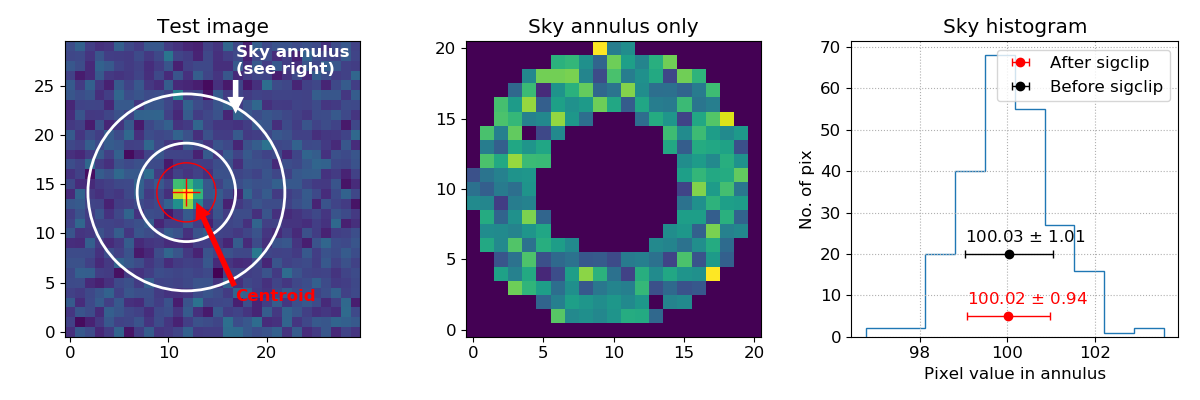
\includegraphics[width=\linewidth]{figs/phot_ap_ex02}
\caption{Left: The test image. Centroid is determined by \cref{eq: centroid} and annulus is defined as $ r_\mathrm{in} = 5 $ and $ r_\mathrm{out} = 10 $ pixels, respectively. Middle: Plotting the sky annulus region only, to just visualize the random fluctuations in the sky region. Clearly, there is no radial trend and it seems quite symmetric along the azimuth. Right: The histogram of the sky pixel values in the annulus. The red/black markers are the median and sample standard deviation of the sky values after and before sigma-clipping, respectively. The sigma clip was done with 3-sigma 50-iterations.}
\label{fig:photapex02}
\end{figure}

Consider we obtained the sky value $ m_\mathrm{sky} $ somehow, e.g., median of sky, \cref{eq: mmm sex} after sigma-clipping, etc. There can be many ways to estimate the uncertainties of this $ m_\mathrm{sky} $. Let me call this $ \Delta m_\mathrm{sky} $. The fluctuation of sky value can critically affect the final result of the photometry. But once a robust way to estimate the sky is set and if the target is bright enough, the uncertainty due to the sky value is not so large. Thus, people do not care too much about the accurate pdf of the $ m_\mathrm{sky} $ value. The most widely used way is to use the practical CLT (Thm \ref{thm: practical clt}) to $ m_\mathrm{sky} $, treating as if it is the mean of the sky samples (although we almost never use the mean for $ m_\mathrm{sky} $). Then
\begin{equation}\label{eq: err m_sky}
  \Delta m_\mathrm{sky} = \frac{s_\mathrm{sky}}{\sqrt{n_\mathrm{sky}}} ~.
\end{equation}
Here, $ s_\mathrm{sky} $ and $ n_\mathrm{sky} $ are the sample standard deviation and the number of the sky pixels survived after the sigma-clipping, respectively. So we are assuming here that the mode has similar uncertainty as the mean.




\subsection{Source Extractor Sky}
We will not cover Source Extractor (SE or SEx or SExtractor) deeply. But simply put, it works like the description below. Say we have the image of 1000 by 1000 pixel.

\begin{enumerate}
\item \textbf{Meshing}: Chop the image by given box size. For example, if you set the box size as $ (50, 25) $, 20 by 40 (in total 800) ``pads'' or ``meshes'' will be made. Each pad will of course have 50 by 25 (in total 1250) pixels.
\item \textbf{Filtering}: Determine the size of the median filter. If the size is $ (3, 3) $, for instance, a 3 by 3 median filter will be used to reduce sharp noised pixels in each pad (similar to Gaussian convolution). The filter size should be determined as a function of seeing disc size. 
\item \textbf{Rejecting Meshes}: In this median-filtered pad, the sigma-clipping is done. If too many pixels inside a pad is rejected, that pad is rejected for the next background estimation step. Such a threshold, say exclusion percentile, must be given by the user. For example, if that percentile is 10 \%, any of the 800 mesh which rejected more than 10 \% of its pixels from sigma-clipping (10 \% out of 1250 pixels, i.e., 125 pixels) will be regarded as ``bad region'' for the sky estimation.
\item \textbf{Sky at each Mesh} (bottom middle panel of \cref{fig:sexbkg01}): Now come back to the original un-filtered meshes. From the pixel values, estimate the sky value and its uncertainty following \cref{eq: mmm sex} and the description below the equation. For the meshes which are flagged as ``bad'' from previous step are not used for this process. As a result, you will have 20 by 40 array of sky values, while some elements may be empty or NaN, if some meshes are flagged ad ``bad''.
\item \textbf{Interpolation} (top middle panel of \cref{fig:sexbkg01}): From the estimated single sky value at each mesh, i.e., the 20 by 40 array, we do interpolation to estimate the sky at all the 1000 by 1000 pixels. The estimation uncertainties should also be calculated for each pixel.
\end{enumerate}

\begin{figure}[ht!]
\centering
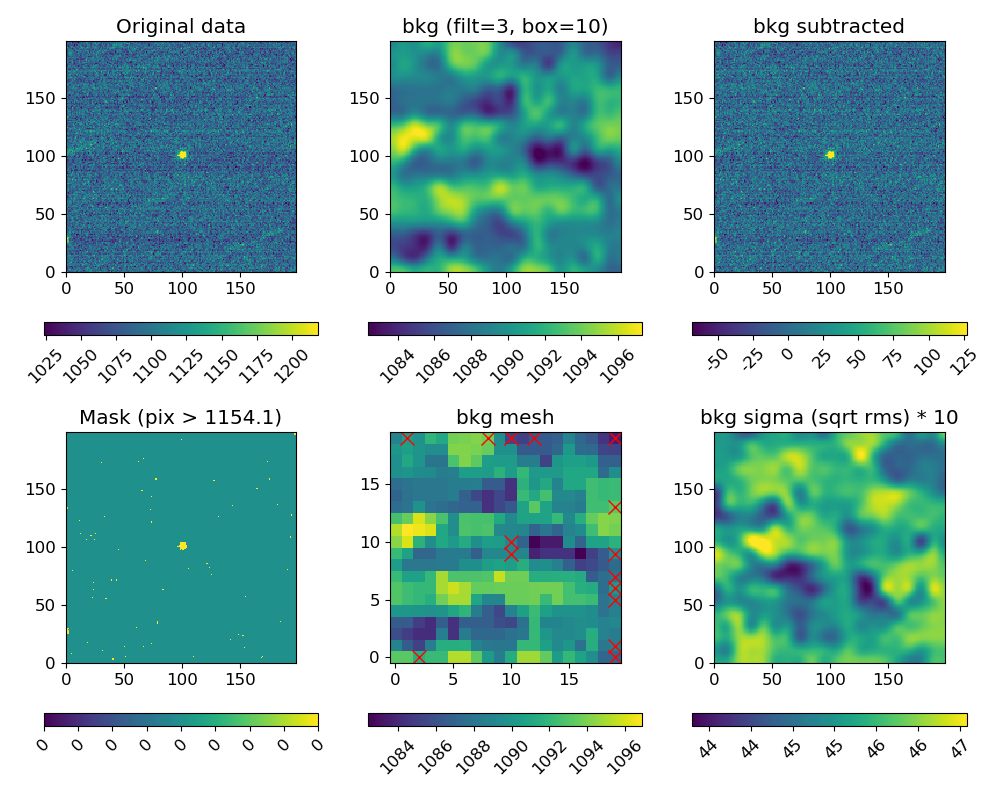
\includegraphics[width=\linewidth]{figs/sex_bkg_01}
\caption{Example of the SExtractor background estimation usage. The original data is the targeto-centric combined image from 13 KMTNet images from SAAO observatory. The pixels with value 1154.1, which is the $ \mathrm{med} + 3\mathrm{std} $ after the sigma-clipping (3-sigma, 5-iter clipping) are masked because those can be stars (bottom left). The background meshes with the estimated sky values (\cref{eq: mmm sex}) are shown in bottom center, and the interpolated one is given in top middle. Note that the sky level changes at maximum around 12 ADU out of the pixel value 1000+. Normally this should be smaller like 5 ADU or 2 ADU within this small region (200 by 200 pixel). The background sigma shown in bottom right is around 4 ADU (note the figure is 10 times the sigma), but many times the sky sigma is smaller than this.}
\label{fig:sexbkg01}
\end{figure}

After the sky subtraction, I plotted the Box plot of the image with x-axis 70 to 90 and y-axis 50 to 150 (python indexing) in \cref{fig:sexbkg02skyhist}.

\begin{figure}[ht!]
\centering
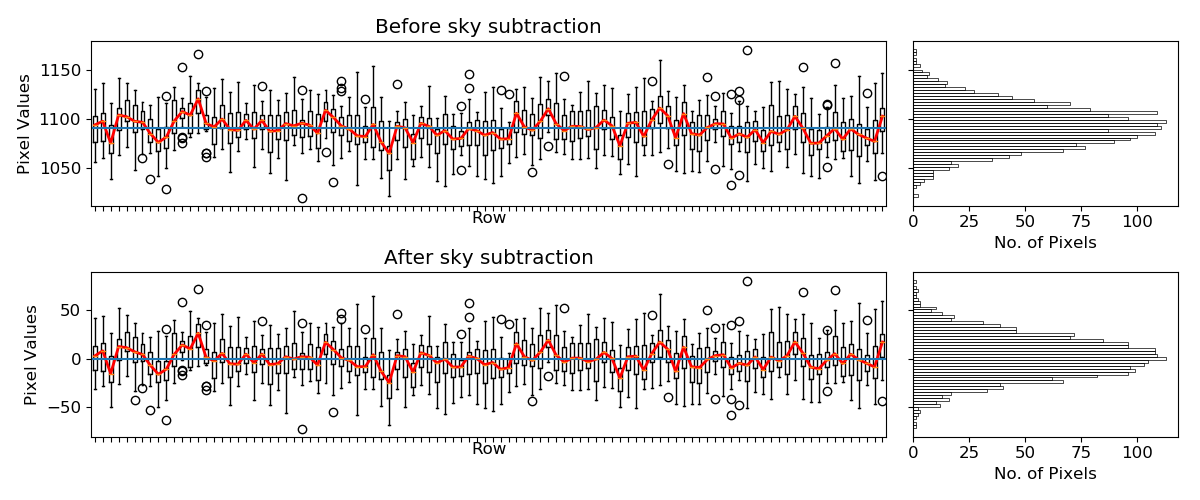
\includegraphics[width=\linewidth]{figs/sex_bkg_02_skyhist}
\caption{The Box plot and pixel value histogram of before/after the sky subtraction, of a region defined by \texttt{data[50:150, 70:90]} (python indexing). The horizontal axes of Box plots correspond to the ``row'' or the y index. Blue horizontal lines are the median of all the pixels in that region, and red solid lines are the medians }
\label{fig:sexbkg02skyhist}
\end{figure}

As can be noticed, SEx background estimation\footnote{We tend to call ``background'' rather than ``sky'' when we are dealing with SExtractor.}, unlike the annulus sky estimation technique, is estimating the sky values at all the pixels, not for each source. Thus, it takes much longer time. Also you can see that lots of parameters (rejection percentile, box size, filter size, interpolation method and related parameters, etc) should be set for SEx to work! In some cases, astronomers run SExtractor again and again to do get expected results, and find best combination of such parameters. But these parameters of course depend on the instruments, sky conditions, etc, so if the results are suspicious, some fine tuning must be made or you have to find different ways to do photometry than SExtractor.


\section{Aperture Shape in Real Reduction}
We most frequently use circular aperture photometry. To determine how large the aperture should be, we need information about the radial profile of the PSF. Historically, there are three important radial profiles: Gaussian, Moffat, and Penny:
\begin{enumerate}
\item \href{https://en.wikipedia.org/wiki/Gaussian_function}{Gaussian}. The Gaussian function.
\item \href{https://en.wikipedia.org/wiki/Moffat_distribution}{Moffat}. A purely empirical function. 
\item Penny. A purely empirical function.
\end{enumerate}
(links to Wikipedia)

Among parameters for PSFs, one that is very widely used in astronomy is the FWHM (full width at half-maximum), as described before. FWHM is defined as the distance between the two points which have the value $\frac{1}{2} f_\mathrm{max}$, i.e., $ f(r = \mathrm{HWHM}) = \frac{1}{2} f_\mathrm{max} $ for $ \mathrm{HWHM} = \mathrm{FWHM}/2 $. FWHM is also used for Lorenzian profile, which has infinite standard deviation (the second centered moment diverges, so the standard deviation is not defined, but FWHM can). The profiles of PSFs and their FWHMs are described below.

In the descriptions below, I will assume the center $ \textbf{r}_0 $ is clearly fixed and the PSF is azimuthally symmetric (circular) and thus $ r = \abs{\textbf{r} - \textbf{r}_0} $ is the only free parameter except for other parameters described in the model.

\subsection{Gaussian}
The circular, i.e., azimuthally symmetric Gaussian PSF is like this:
\begin{equation}\label{eq: profile gauss}
  f_\mathrm{Gauss}(r|A, \sigma) = A e^{ -r^2 / 2\sigma^2 } 
\end{equation}
Here, $r$ is the distance from the center ($r_0$), and $\sigma$ is the standard deviation of the profile. This is the most famous form when it comes to numerical calculation, because all the normalization constants are not so important in PSF fitting.

The normalization constant $A = \qty( \frac{1}{\sqrt{2 \pi \sigma^2}} )^N$ for an $ N $-D Gaussian, such that the integration is normalized, i.e., $ \int_{-\infty}^{+\infty} f_\mathrm{Gauss}(r) 2\pi r dr = 1$. The 2-D Gaussian of integrated flux $ I $ is, therefore,
\begin{equation}\label{eq: profile gauss flux}
  f_\mathrm{Gauss}(r|I, \sigma) = \frac{I}{2 \pi \sigma^2} e^{ -r^2 / 2\sigma^2 }
\end{equation}
This is useful because the total integrated flux is an input parameter. Conversion between this and \cref{eq: profile gauss} is very easy.

The FWHM is calculated by setting $f_{\rm Gauss}(r = \mathrm{HWHM}) = \frac{A}{2}$. First we obtain $ (\mathrm{HWHM})^2 = (2 \ln 2) \sigma^2 $ and thus,
\begin{equation}\label{eq: FWHM gauss}
  \mathrm{FWHM (circ Gauss)} := 2 \sqrt{2 \ln 2} \sigma ~.
\end{equation}

Re-formulating \cref{eq: profile gauss flux} with FWHM ($ F $ for brevity):
\begin{equation}\label{eq: profile gauss fwhm}
  f_{\rm Gauss}(r|I, F) = I \frac{4\ln 2}{\pi F^2} e^{ - (4 \ln 2) r^2 / F^2 } ~.
\end{equation}
This is not widely used, although both $ I $ and $ F $ are what we're most interested in. Rather, people tend to convert $ F $ to $ \sigma $ and use \cref{eq: profile gauss} or \cref{eq: profile gauss flux}.

\subsection{Moffat}
The first suggestion of using Moffat profile was made in 1969 by A. F. J. Moffat in \href{https://ui.adsabs.harvard.edu/abs/1969A\%26A.....3..455M}{Moffat AFJ 1969, A\&A, 3, 455}. It is purely an empirical function, and is one of the most widely accepted form, because of its simple form yet powerful in fitting many circular profiles. Comparison of notations is given in \cref{tab: Moffat}.

\begin{table}
\label{tab: Moffat}
\caption{Moffat profile comparison. \texttt{astropy}'s notation is strikingly confusing, because of its \texttt{alpha} notation, which completely goes against the original Moffat paper and other software implementations (e.g., IRAF). Note: \texttt{AsPyLib} is developed by J. Caron in Python 2 and the development is halted since 2013.}
\centering
\begin{tabular}{cccl}
  \hline
  Symbol &
  \href{http://docs.astropy.org/en/stable/api/astropy.modeling.functional_models.Moffat2D.html\#astropy.modeling.functional_models.Moffat2D}{astropy} & 
  \href{https://iraf.net/irafhelp.php?val=psfmeasure&help=Help+Page}{IRAF}, \href{http://www.aspylib.com/doc/aspylib_fitting.html}{AsPyLib} & 
  Description \\
  \hline
  $ r $ & & & radial distance from the center ($ r_0 = (x_0, y_0) $) \\
  $ R $ & \texttt{gamma} & \texttt{alpha} & core width \\
  $ \beta $& \texttt{alpha} & \texttt{beta} & power \\
  \hline
\end{tabular}
\end{table}

The circular, i.e., azimuthally symmetric Moffat PSF is:
\begin{equation}\label{eq: profile moffat}
  f_\mathrm{Moffat} (r|A, R, \beta) = A \left [ 1 + \left ( \frac{r}{R} \right )^2 \right ]^{-\beta} ~.
\end{equation}
The parameter $R$ is called the core width and $\beta$ is called the power. As in Gaussian case, this is the most widely used form in numerical calculation.

Normalizing as we did for Gaussian, $ \int_{-\infty}^{+\infty} f_\mathrm{Moffat}(r) 2\pi r dr = 1 $, we have the constant $ A = \frac{\beta - 1}{\pi R^2} $. Therefore, Moffat profile has a restriction that $ \beta > 1 $. The Moffat profile for the integrated flux $ I $ is, similar to Gaussian,
\begin{equation}\label{eq: profile moffat flux}
  f_\mathrm{Moffat}(r|I, R, \beta) = I \frac{\beta - 1}{\pi R^2} \left [ 1 + \left ( \frac{r}{R} \right )^2 \right ]^{-\beta}
\end{equation} 
Similar to Gaussian, this is also widely used.

The FWHM is calculated by setting $f_\mathrm{Moffat}(\mathrm{HWHM}) = \frac{A}{2}$. As we did in Gauss example, we obtain $ \mathrm{HWHM}^2 = R^2 (2^{1/\beta}-1) $,
\begin{equation}\label{eq: FWHM moffat}
  \mathrm{FWHM}(\mathrm{circMoffat}) = 2 R \sqrt{2^{1/\beta}-1} ~.
\end{equation}

Using FWHM ($ F $ for brevity), we re-formulate Moffat profile \cref{eq: profile moffat flux}\footnote{\href{https://ui.adsabs.harvard.edu/abs/2001MNRAS.328..977T/abstract}{Trujillo+2001, MNRAS, 328, 977}}:
\begin{equation}\label{eq: profile moffat fwhm}
  f_\mathrm{Moffat}(r|I, F, \beta)
    = I \frac{4(2^{1/\beta} - 1) (\beta - 1)}{\pi F^2}
      \left [ 1 + 4(2^{1/\beta} - 1) \left ( \frac{r}{F} \right )^2 \right ]^{-\beta} ~.
\end{equation}

\begin{thm}[High power Moffat is Gaussian]
For $ \beta \rightarrow \infty $,
\begin{equation}
  f_{\rm Moffat} (r|I, F, \infty) = f_{\rm Gauss}(r|I, F) ~.
\end{equation}
Practically $ \beta \gtrsim 100 $ is enough for this approximation.
\end{thm}
\begin{proof}[of Thm]
For $ \beta \rightarrow \infty $, we approximate $ 2^{1/\beta} - 1 \approx \frac{\ln 2}{\beta} $, so
\begin{equation*}
  f_\mathrm{Moffat}(r|I, F, \infty)
    \approx I \frac{\tilde{A}}{\pi} 
      \lim_{\beta \rightarrow \infty} \frac{\beta-1}{\beta} 
      \left [ 1 + \frac{\tilde{A} r^2}{\beta} \right ]^{-\beta} ~,
\end{equation*}
for $ \tilde{A} = \frac{4 \ln 2}{F^2} $. Note that $ \lim_{\beta \rightarrow \infty} \left [ 1 + \frac{\tilde{A}}{\beta} \right ]^{-\beta} \equiv e^{-\tilde{A}} $ and $ \frac{\beta-1}{\beta} $ becomes unity. Substituting these, we get the approximated formula identical to \cref{eq: profile gauss fwhm}, or to \cref{eq: profile gauss} with \cref{eq: FWHM gauss}. Q.E.D.
\end{proof}

Also, if you look at the pdf of the Students' $ t $-distribution, Moffat is a special case of the $ t $-distribution, but with a simpler re-parameterization (original $ t $-distribution has a clear mathematical reason why it appeared, but it has normalization constants including the Gamma functions, etc, so computationally a bit more complicated). 

\subsection{Penny}
It was Franz\footnote{ \href {https://ui.adsabs.harvard.edu/abs/1973JRASC..67...81F/abstract} {FranzOG 1973, JRASC, 67, 81}}, who first used Lorenzian-like profile for stars. Then Penny\footnote{ \href {https://ui.adsabs.harvard.edu/abs/1979MNRAS.187..829P/abstract} {PennyAJ 1979, MNRAS, 187, 829}} used it with linear interpolation in sky level to do the UBV photometry for visual binaries close to each other. After that, Penny and Dickens\footnote{ \href {https://ui.adsabs.harvard.edu/abs/1986MNRAS.220..845P/abstract} {PennyAJ \& DickensRJ, 1986, MNRAS, 220, 845}, which is cited for more than 110 times as of Oct 2019}, using their own package (\texttt{STARMAN}), introduced Gaussian and Lorentzian mixed model\footnote{Unfortunately, however, both the original Penny \& Dickens paper and \href{https://ui.adsabs.harvard.edu/abs/1995StaUN.141.....P/abstract}{Penny (1995, StaUN 141)} pp.44--45 have so many typos in the star profile formulae...}. 

The original profile suggested by Penny is a sum of a circular Gaussian and elliptical modified-Lorentzian:
\begin{equation}\label{eq: profile penny}
  \begin{aligned}
    f(r &| A, Q, \sigma_1, \sigma_2, \sigma_3, \sigma_4, P, \theta, P_Q, R_Q)  \\
    &= A 
      \left \{ 
        \frac{1}
        {1 + \left[ 
          \left( \frac{x'}{\sigma_1} \right)^2 
          + \left( \frac{y'}{\sigma_2} \right)^2 
          \right ]
          ^{\frac{P}{2} 
            \left( 1 + \sqrt{\left( \frac{x'}{\sigma_3} \right)^2 
              + \left( \frac{y'}{\sigma_4} \right)^2 } \right) 
           }}
        + Q \exp \left [ - \left ( \frac{r}{R_Q} \right )^{P_Q} \right ]
      \right \}
  \end{aligned} ~,
\end{equation}
for
\begin{equation*}
  \binom{x'}{y'} = \binom{x_0}{y_0} 
  + \mqty(\cos \theta & \sin \theta \\ -\cos \theta & \sin \theta) \binom{x}{y}
\end{equation*}
where $ \textbf{r}_0 = (x_0, y_0) $ is the center, and $ \theta $ is the tilting angle of the Lorentzian. The notation $ \sigma_{1,2,3,4} $ are $ R_\mathrm{maj} $ (\texttt{RX}), $ R_\mathrm{min} $ (\texttt{RY}), $ RP_\mathrm{maj} $ (\texttt{PRX}), and $ RP_\mathrm{min} $ (\texttt{PRY}) in the \texttt{POORMAN}'s notations. It is no more widely used, because of the large number of free parameters.

In IRAF, it is implemented\footnote{The source code is at \href {https://github.com/iraf-community/iraf/blob/master/noao/digiphot/daophot/daolib/profile.x} {\texttt{noao.digiphot.daophot.dailib.profile.x}}.} in two ways: \texttt{penny1} and \texttt{penny2}. 



\footnote{Although there is no reference, ``Photometry using IRAF v. 2.5.1'' (2012-03-25) by Keunhong Park, Jinhyuk Ryu, Insung Jang, and Ho Seong Hwang notes that (p. 8): ``\texttt{penny1} or \texttt{penny2} of IRAF fits the analytical stellar profiles well, while \texttt{moffat15} or \texttt{moffat25} fits the stellar profiles well if observed on cloudy nights.'' I cannot even understand the meaning of it...}

Simple way of using it is, assuming $ Q = 0 $, $ P = 2 $, and $ \sigma_3, \sigma_4 \rightarrow \infty $, so that
\begin{equation}\label{eq: profile penny12}
  f(r|A, \theta, \sigma_1, \sigma_2, 
\end{equation}




\subsection{IRAF}
Here I describe how IRAF does centroiding in its \href{https://iraf.net/irafhelp.php?val=imexam&help=Help+Page}{IRAF \texttt{imexamine} task}. It is crude but always works decently, so I thought it's a good idea to summarize it for benchmark purpose\footnote{The description below is the description of IRAF \texttt{imexamine} when you hit \texttt{a} key on IRAF. Since \texttt{imexamine} is not only for the 2-D analysis, it consists of parameters for the 1-D extraction (when you hit \texttt{j} or \texttt{k}), for instance. You may want to fit a Gaussian to the pixels along a vertical line (i.e., $ N \times 1 $ array). For those purposes, \texttt{imexamine} has more parameters like \texttt{sigma}, etc. Please don't be confused when you read the doc.
}.

First, set $ r $, the circular aperture radius (default \texttt{radius=5}). Then the sky level is determined from an annulus with the inner radius \texttt{radius+buffer} (default \texttt{buffer=5}) and the outer radius \texttt{radius+buffer+width} (default \texttt{width=5}), centered at the initial center position. By default (\texttt{xorder=0}, \texttt{yorder=0}), the sky value is set as the median value in this annulus. If both of \texttt{xorder} and \texttt{yorder} are larger than 0, then the 2-D polynomial of these orders is fitted to the pixel values from the annulus. Mathematically speaking, \texttt{xorder=yorder=1} means a constant value (the weighted average value). 

Then the centering is done by fitting 1-D Gaussian or Moffat to the marginalized pixel values (default is Moffat by \texttt{fittype="moffat"}), for the square box with $ \mathrm{width} = \mathrm{height} = 2r $.  In pythonic way, you are fitting 1-D profile to \pyth{np.sum(data, axis=0)} and \pyth{np.sum(data, axis=1)} to get the y and x centers, respectively. The pixels below the average value in this box are masked in the centering process\footnote{Not clear from the doc: How are the weighting scheme applied in this 1-D profile fittings? As in the 2-D profile fit? Or no error-bars?}. 

It is repeated for certain times (default \texttt{iterations=3}), until the updated center position resides in the same pixel as the previous step\footnote{Not clear from the doc: I worried what if the center position is at the edge of the pixel. I guess, maybe, even though the center position is updated from the right edge of the $ i $-th to the left edge of the $ (i+1) $-th pixel, the centering box will remain the same in the upcoming iterations, so the centering process will be halted (converged) at the left edge of the $ (i+1) $-th pixel.}. In every iteration, the aperture radius $ r $ is updated to $ 3\, \mathrm{FWHM} $ using the FWHM obtained from the last iteration (from this definition, $ r $ remains as the initial value if \texttt{iterations=1}). Any pixel outside the image will be assumed to have a constant value (default \texttt{constant=0}). 

The weighting for each pixel is calculated by
\begin{equation}\label{eq: imexam weighting}
  w (r_{\texttt{i,j}}) = \left \{ 
  \begin{array}{cr}
    r_\mathtt{i,j}^{-2} & r_\mathtt{i,j} \le \mathrm{FWHM}/2 \\
    e^{-\left ( \frac{r_\mathtt{i,j}}{\mathrm{FWHM}/2} - 1 \right )^2} & r_\mathtt{i,j} > \mathrm{FWHM}/2
  \end{array}
  \right . ~,
\end{equation}
where $ \mathrm{FWHM}/2 $ is also called $ \mathrm{HWHM} $ or $ r_\mathrm{half} $ and $ r_\mathtt{i,j} $ is the distance in pixel unit to the \texttt{(i, j)}-th pixel from the center\footnote{Not clear from the doc: Center of the last iteration?}. This weighting scheme is different from usual least square statistic (which uses $ w = 1/\sigma^2 $). 

Once this fitting is done, put a circular aperture with radius $ r $. Because the purpose of \texttt{imexamine} is not an accurate photometry, it crudely estimates the flux by summing the pixel values for pixels which has its center within the aperture (same as putting \pyth{method="center"} to photutils aperture). 

Two more parameters are calculated, namely, ellipticity $ e $ and angle $ \mathrm{pa} $:
\begin{equation}
  e = \sqrt{\frac{ (M_{xx} - M_{yy})^2 + 4 M_{xy}^2}{M_{xx} + M_{yy}}}
  \quad;\quad
  \mathrm{pa}
    = \frac{1}{2} \atan(\frac{2 M_{xy}}{M_{xx} - M_{yy}}) ~,
\end{equation}
where the moments
\begin{equation}
  M_\mathtt{ij} = \frac{\sum I \times i \times j}{\sum I}
\end{equation}
for pixel value $ I $ and $ i, j \in [x, y] $. 



In realistic photometry, such as \href{https://iraf.net/irafhelp.php?val=psfmeasure&help=Help+Page}{IRAF \texttt{psfmeasure} task}, we must use $ I - \mathrm{sky} $ instead of $ I $. 

Some old packages including \texttt{ROMAFOT}, \texttt{STARMAN}, \texttt{DAOPHOT}, \texttt{DoPHOT}, \texttt{WOLF}, \texttt{LUND}, \texttt{CAPELLA} are summarized in \href{http://web.ipac.caltech.edu/staff/fmasci/home/astro_refs/WhyPSFfit.pdf}{this lecture note} and \href{https://ui.adsabs.harvard.edu/abs/1992ASPC...25..297S/abstract}{StetsonPB 1992, ASPC, 25, 297}


\subsubsection*{Note}
The shape of circular apetures were briefly discussed. In reality, you may encounter apertures of ellipse, box, pill-box, or any other scientifically meaningful ones. Now what you have to understand more is the aperture \emph{size}.

\section{Aperture Size in Real Reduction}
We will stick to the circular apertures here, too. Any other compilcated apertures may have to be used depending on the scientific reasons. Here I will describe three \emph{ideas} of finding the aperture size. When you have to apply aperture size in professional research, these should not be used blindly, but you have to find your own way which is both mathematically robust and scientifically meaningful for your specific purpose.

\subsection{Maximum SNR (not recommeneded)}
The singal-to-noise ratio is a 


\subsection{Growth Curve (mathematically robust)}
Stetson 1988 PASP






